\chapter{Common Methodological Framework}
\label{ch:framework}

Chapter~\ref{ch:dataset} established the structure and constraints of the
available data. This chapter describes the methodological framework that
the project's successive implementation phases used, with variation, to
work within those constraints. Rather than repeating a phase-by-phase
account here, it extracts the building blocks that recur across phases —
evaluation regimes, representation strategies, model families, metrics,
and the treatment of remaining-useful-life — so that
Chapter~\ref{ch:activities} can describe each phase's activity without
re-explaining shared machinery, and so that later comparisons
(Chapter~\ref{ch:results}) can be made on a consistent methodological
footing.

\section{General Modelling Philosophy}
\label{sec:philosophy}

The project's successive phases addressed several distinct prediction
problems over the same underlying dataset: estimating a specimen's current
visible-corrosion state from an image; predicting a specimen's terminal
structural condition; fitting an exploratory model of how corrosion and
structural condition evolve over time; screening for an approximate
service-life indicator; and, in a later and separate effort, classifying
images into a discrete visible-corrosion severity category. These are not
variations on a single problem, and the report does not treat them as such.

What is shared across phases is not the prediction target but a
methodological principle that later phases articulated increasingly
explicitly: a claim made about the data must correspond to the
supervision the data actually provides. A model trained on dense
visible-corrosion labels supports claims about visible-corrosion
estimation; it does not, by itself, support claims about structural
condition, service life, or failure risk, however plausible an
extrapolation from corrosion to those quantities might seem. The
distinctions drawn in Section~\ref{sec:dataset-summary} between directly
observed, model-derived, and derived-screening quantities are the
practical expression of this principle, and Section~\ref{sec:proxy-rul}
returns to its most consequential application.

\section{Leakage-Safe Specimen-Level Evaluation}
\label{sec:leakage}

Section~\ref{sec:longitudinal} established that the repeated image
observations of a given specimen are correlated rather than independent.
This has a direct and easily overlooked consequence for evaluation.

Consider a dataset of image observations split into training and test
partitions by assigning individual image rows at random, without regard
to which specimen each row belongs to. Because a typical specimen
contributes fifteen to eighteen images spanning its entire observation
period, a random row-wise split will, with high probability, place most
of a given specimen's images in the training partition and a few of the
same specimen's images in the test partition. A model evaluated in this
way can achieve a low test error not by learning corrosion cues that
generalise to specimens it has never seen, but by learning to recognise
that specific specimen — its particular lighting, its particular
background, or idiosyncrasies of its individual corrosion pattern — from
the many other images of it already seen in training. The resulting test
error understates the error the same model would incur on a genuinely
unseen specimen, and the extent of this understatement is not visible from
the row-wise test score alone.

The project's later implementation phases addressed this by grouping
observations at the specimen level before splitting: every image
belonging to a given specimen is assigned to the same partition, so that a
specimen appearing in the test partition never also appears in training.
Figure~\ref{fig:specimen-splitting} contrasts the two approaches. This
grouping principle is applied consistently, regardless of which of the
three evaluation regimes described next is used to decide which specimens
are held out.

\begin{figure}[htbp]
\centering
\resizebox{0.75\textwidth}{!}{% Report schematic (not an experimental result).
% Contrasts a naive row-wise random split of image observations against
% a specimen-level grouped split, for four illustrative specimens A-D
% each with several repeated image observations.
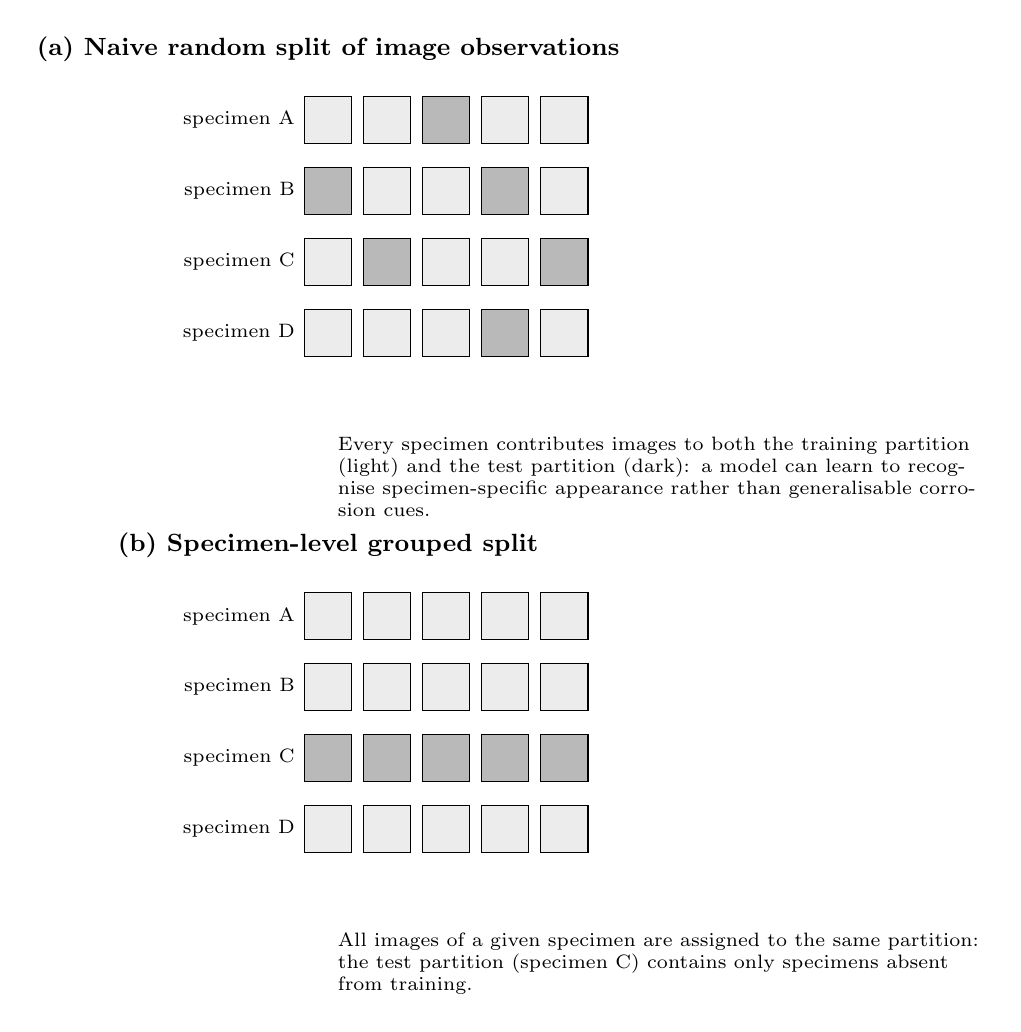
\begin{tikzpicture}[
    sq/.style={draw, minimum size=6mm, inner sep=0pt, font=\tiny},
    train/.style={sq, fill=gray!15},
    test/.style={sq, fill=gray!55},
    lbl/.style={font=\scriptsize, anchor=east},
    panelcap/.style={font=\small\bfseries}
]

% --- Panel (a): naive random row-wise split ---
\node[panelcap] at (0,0) {(a) Naive random split of image observations};

\foreach \row/\name/\pattern [count=\r from 0] in
    {0/A/{train,train,test,train,train},
     1/B/{test,train,train,test,train},
     2/C/{train,test,train,train,test},
     3/D/{train,train,train,test,train}} {
    \node[lbl] at (-0.3,-0.9-\r*0.9) {specimen \name};
    \foreach \p [count=\c from 0] in \pattern {
        \node[\p] at (\c*0.75,-0.9-\r*0.9) {};
    }
}
\node[font=\scriptsize, align=left, text width=8.2cm, anchor=north west]
    at (0,-4.8) {Every specimen contributes images to both the training
    partition (light) and the test partition (dark): a model can learn to
    recognise specimen-specific appearance rather than generalisable
    corrosion cues.};

% --- Panel (b): specimen-level grouped split ---
\begin{scope}[yshift=-6.3cm]
\node[panelcap] at (0,0) {(b) Specimen-level grouped split};

\foreach \row/\name/\assign [count=\r from 0] in
    {0/A/train,1/B/train,2/C/test,3/D/train} {
    \node[lbl] at (-0.3,-0.9-\r*0.9) {specimen \name};
    \foreach \c in {0,...,4} {
        \node[\assign] at (\c*0.75,-0.9-\r*0.9) {};
    }
}
\node[font=\scriptsize, align=left, text width=8.2cm, anchor=north west]
    at (0,-4.8) {All images of a given specimen are assigned to the same
    partition: the test partition (specimen C) contains only specimens
    absent from training.};
\end{scope}

\end{tikzpicture}
}
\caption{Report schematic contrasting a naive row-wise random split, which
can place images of the same specimen on both sides of a train/test
partition, against a specimen-level grouped split, which cannot. Not an
experimental result.}
\label{fig:specimen-splitting}
\end{figure}

\section{Evaluation Regimes}
\label{sec:eval-regimes}

Specimen-level grouping determines that whole specimens, not individual
images, are the unit of assignment to a partition. It does not by itself
determine \emph{which} specimens are held out, or what question the
resulting evaluation answers. The project uses three distinct regimes for
this purpose, each targeting a different question, summarised in
Table~\ref{tab:eval-regimes} and illustrated schematically in
Figure~\ref{fig:eval-regimes}.

\subsection{Grouped specimen holdout}
\label{sec:grouped-holdout}

A random subset of specimens is held out from the pooled observed dataset
without deliberately withholding an entire treatment or campaign. It
therefore provides an interpolation-oriented unseen-specimen evaluation,
answering the question of how well a model generalises to specimens it
has not seen, drawn at random from the same pooled experimental mixture
it was trained on. This is distinct from stratified sampling: because the
subset is drawn at random rather than balanced by design, individual
folds may be imbalanced in campaign or treatment composition and need not
contain every subgroup. It is the regime closest to ordinary interpolation
within the observed design space, and, where repeated evaluation is used,
results are averaged over multiple random selections of the held-out
subset.

\subsection{Leave-one-treatment-out}
\label{sec:loto}

All specimens sharing a given treatment protocol are held out together,
cycling over the available treatment groups so that every group is used
as the test partition exactly once. This answers a more demanding
question: whether a model's predictions transfer to a treatment protocol
it has never encountered at all, rather than merely to unseen specimens of
protocols it has already seen examples of. Because some treatment groups
are represented by very few specimens (Table~\ref{tab:campaign-design}),
individual leave-one-treatment-out folds can be based on small held-out
samples, and results for the smallest groups are correspondingly less
stable.

\subsection{Leave-one-campaign-out}
\label{sec:loco}

All specimens belonging to one full experimental campaign are held out,
and the model is trained on the other campaign alone. This is the
strongest distribution shift the dataset can express, since, as
established in Section~\ref{sec:confounding}, campaign identity coincides
with a specific combination of steel-mesh configuration, chloride
concentration, and terminal ageing duration. A model evaluated under
leave-one-campaign-out is therefore not being tested on specimens drawn
from the training distribution; it is being tested on specimens whose
design characteristics differ systematically, along several correlated
dimensions at once, from every specimen available for training. For this
reason, leave-one-campaign-out performance in this dataset should not be
read as an estimate of expected performance on future, similarly-designed
specimens; it is better understood as a stress test of extrapolation
across the experimental design space, and the two readings can differ
substantially. This report does not present leave-one-campaign-out results
in this chapter — the regime is defined here only as a methodological
tool; its results, and what they imply, are discussed once the relevant
modelling activities are described in Chapters~\ref{ch:activities}
and~\ref{ch:results}.

\begin{table}[htbp]
\centering
\caption{The three specimen-level evaluation regimes used across the
project, and the question each is designed to answer.}
\label{tab:eval-regimes}
\begin{tabular}{p{3.6cm}p{3.6cm}p{6.2cm}}
\toprule
Regime & Held-out unit & Question answered \\
\midrule
Grouped specimen holdout & Random subset of specimens & Generalisation to
unseen specimens drawn from the same observed experimental mixture. \\
Leave-one-treatment-out & All specimens of one treatment protocol & Transfer
to a treatment protocol not seen at all during training. \\
Leave-one-campaign-out & All specimens of one full campaign & Robustness
under the strongest available distribution shift; partly an extrapolation
test across correlated design variables (Section~\ref{sec:confounding}). \\
\bottomrule
\end{tabular}
\end{table}

\begin{figure}[htbp]
\centering
\resizebox{0.8\textwidth}{!}{% Report schematic (not an experimental result).
% Illustrates, for a generic grid of specimens organised by campaign
% (rows) and treatment group (columns), which specimens are held out
% as the test partition under each of the three evaluation regimes.
% The layout is illustrative only and does not reproduce the exact
% campaign/treatment specimen counts given in the dataset chapter.
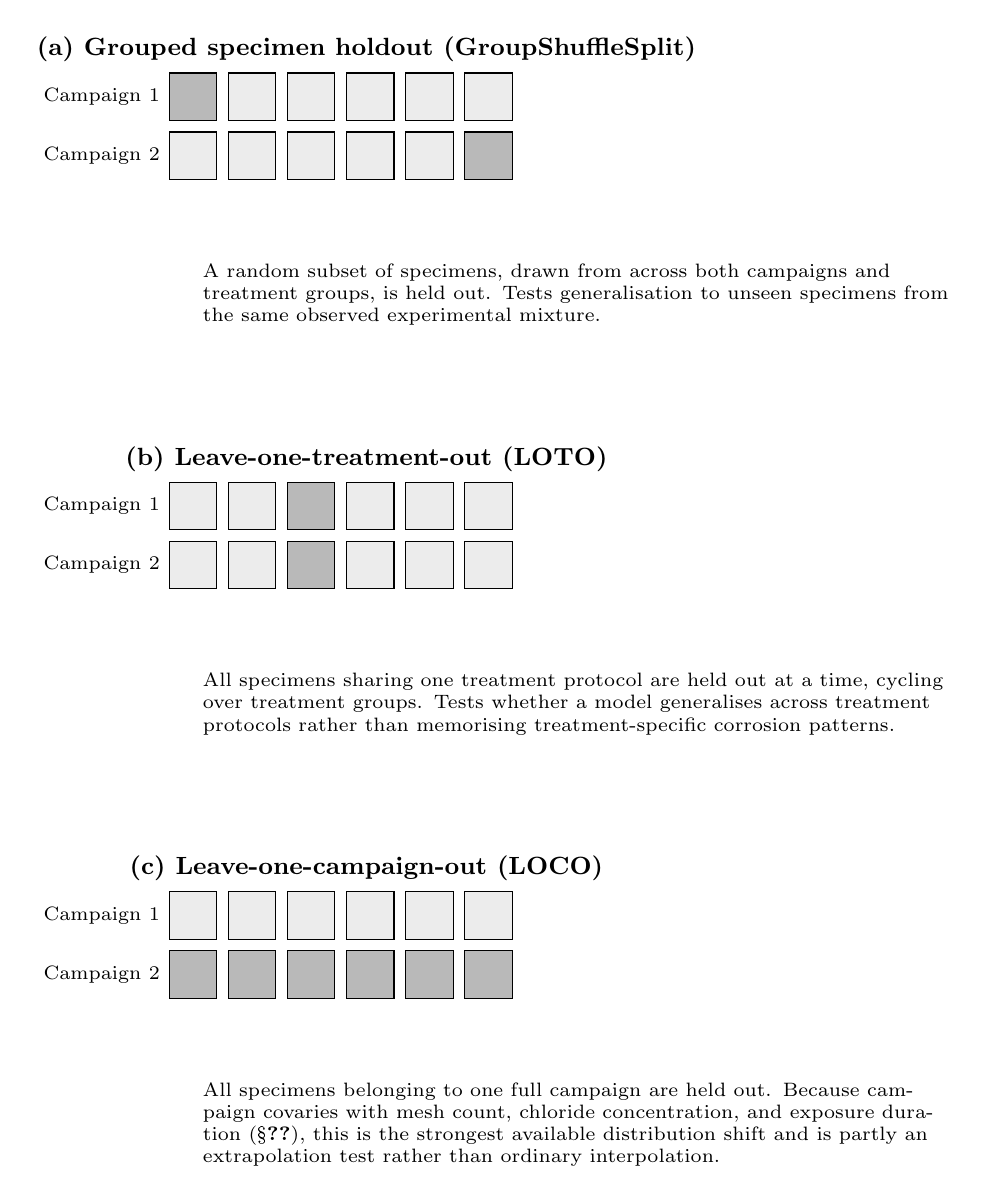
\begin{tikzpicture}[
    sq/.style={draw, minimum size=6mm, inner sep=0pt},
    train/.style={sq, fill=gray!15},
    held/.style={sq, fill=gray!55},
    panelcap/.style={font=\small\bfseries},
    rlbl/.style={font=\scriptsize, anchor=east},
    clbl/.style={font=\scriptsize, anchor=south}
]

\def\ncols{6}

% --- Panel (a): GroupShuffleSplit ---
\node[panelcap] at (2.2,0.6) {(a) Grouped specimen holdout (GroupShuffleSplit)};
\foreach \r/\rowname in {0/Campaign 1, 1/Campaign 2} {
    \node[rlbl] at (-0.3,-\r*0.75) {\rowname};
    \foreach \c in {0,...,5} {
        \pgfmathtruncatemacro{\isheld}{mod(\c+2*\r,7)==0}
        \ifnum\isheld=1
            \node[held] at (\c*0.75,-\r*0.75) {};
        \else
            \node[train] at (\c*0.75,-\r*0.75) {};
        \fi
    }
}
\node[font=\scriptsize, align=left, text width=9.5cm, anchor=north west]
    at (0,-2.0) {A random subset of specimens, drawn from across both
    campaigns and treatment groups, is held out. Tests generalisation
    to unseen specimens from the same observed experimental mixture.};

% --- Panel (b): LOTO ---
\begin{scope}[yshift=-5.2cm]
\node[panelcap] at (2.2,0.6) {(b) Leave-one-treatment-out (LOTO)};
\foreach \r/\rowname in {0/Campaign 1, 1/Campaign 2} {
    \node[rlbl] at (-0.3,-\r*0.75) {\rowname};
    \foreach \c in {0,...,5} {
        \ifnum\c=2
            \node[held] at (\c*0.75,-\r*0.75) {};
        \else
            \node[train] at (\c*0.75,-\r*0.75) {};
        \fi
    }
}
\node[font=\scriptsize, align=left, text width=9.5cm, anchor=north west]
    at (0,-2.0) {All specimens sharing one treatment protocol are held
    out at a time, cycling over treatment groups. Tests whether a model
    generalises across treatment protocols rather than memorising
    treatment-specific corrosion patterns.};
\end{scope}

% --- Panel (c): LOCO ---
\begin{scope}[yshift=-10.4cm]
\node[panelcap] at (2.2,0.6) {(c) Leave-one-campaign-out (LOCO)};
\foreach \r/\rowname in {0/Campaign 1, 1/Campaign 2} {
    \node[rlbl] at (-0.3,-\r*0.75) {\rowname};
    \foreach \c in {0,...,5} {
        \ifnum\r=1
            \node[held] at (\c*0.75,-\r*0.75) {};
        \else
            \node[train] at (\c*0.75,-\r*0.75) {};
        \fi
    }
}
\node[font=\scriptsize, align=left, text width=9.5cm, anchor=north west]
    at (0,-2.0) {All specimens belonging to one full campaign are held
    out. Because campaign covaries with mesh count, chloride
    concentration, and exposure duration (\S\ref{sec:confounding}), this
    is the strongest available distribution shift and is partly an
    extrapolation test rather than ordinary interpolation.};
\end{scope}

\end{tikzpicture}
}
\caption{Report schematic of the three evaluation regimes, for an
illustrative grid of specimens organised by campaign and treatment group.
Held-out (test) specimens are shown in the darker shade. The layout is
illustrative and does not reproduce the exact specimen counts of
Table~\ref{tab:campaign-design}.}
\label{fig:eval-regimes}
\end{figure}

\section{Image Representation Strategies}
\label{sec:representation}

Across its successive phases, the project explored five broad strategies
for converting an image observation into a representation usable by a
predictive model:

\begin{enumerate}
\item[A.] \textbf{Threshold and handcrafted colour descriptors.} A small
number of scalar quantities computed from fixed colour-space thresholds
(for example, the proportion of pixels falling within a rust-coloured
range), used by the earliest implementation phases.
\item[B.] \textbf{Pretrained deep embeddings.} A fixed-length vector
representation obtained by passing each image through a convolutional
network pretrained on a large natural-image dataset and used as a frozen
feature extractor, without further training of the network itself.
\item[C.] \textbf{Interpretable multi-family features.} A broader,
explicitly engineered set of descriptors spanning colour, texture, surface
morphology, and spatial location of corrosion along the specimen, designed
so that each feature has a stated physical or visual interpretation.
\item[D.] \textbf{RGB/HSV summary representations.} Colour-space summary
statistics computed in both RGB and HSV representations, introduced
specifically to test whether a compact, interpretable colour description
adds value once specimen-design metadata is already available, in the
project's terminal-load-focused analysis.
\item[E.] \textbf{Raw-image deep classification (planned).} Direct
classification of raw images into a discrete corrosion-severity category
using a deep image classifier, which is the intended representation
strategy for the later four-class classification effort described in
Chapter~\ref{ch:activities}; at the time of writing, this strategy has been
prepared for (through a dedicated, leakage-safe data and augmentation
pipeline) but not yet trained or evaluated.
\end{enumerate}

These strategies are introduced here only as a taxonomy; the specific
feature definitions used within each strategy are not repeated in this
chapter and, where needed for reference, are catalogued in an appendix.

\section{Metadata and Multimodal Inputs}
\label{sec:multimodal}

A recurring methodological question across phases is whether an
image-derived representation, of any of the strategies above, contributes
predictive information beyond what is already available from specimen and
exposure metadata (Table~\ref{tab:campaign-design}) alone. This question
matters because metadata and image-derived quantities are not, in
general, independent sources of information in this dataset: a specimen's
treatment and campaign membership can itself be predictive of its
corrosion appearance or its structural condition, independently of
whatever a photograph of it shows.

The project's treatment of this question was not uniform across phases,
and the framework below describes how the comparison was eventually
formalised rather than a design followed from the outset. The
deep-embedding phase compared an image-only configuration against a
combined image-plus-metadata configuration, but did not include a
comparable metadata-only baseline alongside them. It was the later
terminal-load-focused work that made an explicit three-way comparison —
an \emph{image-only} configuration using an image representation without
metadata, a \emph{metadata-only} configuration using specimen and exposure
design variables without any image-derived quantity, and a
\emph{combined} (multimodal) configuration using both together — a
central and consistently applied part of its methodology. Where this
three-way comparison is available, it is the project's principal tool for
distinguishing predictive value that is genuinely attributable to the
visual appearance of corrosion from predictive value that is instead
attributable to the specimen's known design and exposure conditions; where
only the narrower two-way comparison is available, this is stated
explicitly alongside the corresponding result. The outcomes of these
comparisons, for the phases in which they were carried out, are reported
in Chapters~\ref{ch:activities} and~\ref{ch:results}.

\section{Model Families}
\label{sec:model-families}

Table~\ref{tab:model-families} lists the model families used across the
project's phases. The choice of family in each phase was pragmatic rather
than exploratory: regularised linear regression provides an
interpretable, low-variance baseline that is particularly informative
when the training sample is small (as it is for the structural targets,
Section~\ref{sec:structural-supervision}); tree-ensemble methods
(Random Forest, Gradient Boosting, XGBoost, CatBoost) provide stronger
non-linear fits with built-in feature-importance diagnostics; a small
multilayer perceptron was used to combine a fixed-length embedding with
tabular metadata; a pretrained convolutional network provided image
embeddings as described in Section~\ref{sec:representation}; and a small
family of parametric and non-parametric curve models was used specifically
to fit specimen-level degradation trajectories over time
(Section~\ref{sec:proxy-rul}). This chapter does not develop the
mathematical detail of any of these families; it records only their role
in the project.

\begin{table}[htbp]
\centering
\caption{Model families used across the project, and their role.}
\label{tab:model-families}
\begin{tabular}{p{4.3cm}p{8.9cm}}
\toprule
Family & Role in the project \\
\midrule
Ridge / linear regression & Regularised, low-variance baseline;
particularly relevant given the small number of structural observations. \\
Random Forest & Non-linear regression and classification baseline with
feature-importance diagnostics; used across most phases and targets. \\
Gradient Boosting & Alternative non-linear ensemble, compared against
Random Forest per task. \\
XGBoost & Alternative gradient-boosted ensemble, benchmarked in the
earliest classical phase and again, alongside other candidate families,
in the later terminal-load-focused modelling. \\
CatBoost & Additional gradient-boosted ensemble candidate introduced in
later structural-condition modelling; used with the same numeric feature
tables as the other ensemble methods, not configured to use its native
categorical-feature handling. \\
Multilayer perceptron (MLP) & Combines a fixed-length image embedding
with tabular metadata; also used as an image-only regressor for
comparison. \\
Pretrained convolutional network & Frozen (not fine-tuned) feature
extractor producing the fixed-length image embedding consumed by the
MLP above. \\
Degradation-curve models & A small family of parametric (linear,
logarithmic, logistic, Gompertz) and non-parametric (monotone-isotonic)
curves fitted to estimated condition over the observation period, as
input to the proxy-RUL computation (Section~\ref{sec:proxy-rul}). \\
\bottomrule
\end{tabular}
\end{table}

\section{Evaluation Metrics}
\label{sec:metrics}

Model performance is reported using a small, consistent set of metrics,
defined here so that later chapters can use them without redefinition.
For regression targets, the project reports the mean absolute error (MAE)
and root-mean-square error (RMSE), both in the physical units of the
target; the coefficient of determination ($R^2$); and the Spearman rank
correlation between predicted and observed values. For the four-class
classification target, the project's planned evaluation (not yet carried
out; Section~\ref{sec:representation}, strategy~E) specifies overall
accuracy, macro-averaged F1 score, and per-class recall reported through a
confusion matrix.

Spearman rank correlation is reported alongside the absolute-error metrics
because it evaluates whether a model correctly orders specimens by
severity without requiring its predictions to be correctly scaled or
calibrated in absolute terms, and because it is markedly less sensitive
than MAE or RMSE to a small number of specimens with large absolute
errors. A model can be poorly calibrated in absolute magnitude while still
correctly identifying which specimens are more severely affected than
others, and the two metrics together distinguish this situation from one
in which a model's ranking of specimens is itself unreliable.

Macro-averaged F1, rather than overall accuracy, is identified in advance
as the primary metric for the planned four-class classification task
because the four severity classes are markedly imbalanced in the
underlying data (Table~\ref{tab:data-modalities}): the lowest-severity
class accounts for the large majority of observations. A classifier that
predicted the majority class for every observation would achieve high
overall accuracy while providing no discrimination among the
minority, higher-severity classes that are of greatest practical
interest. Macro-averaged F1 weights each class equally regardless of its
frequency and is therefore markedly more informative than accuracy alone
for this task; per-class recall and the confusion matrix are reported
alongside it to characterise which classes, specifically, a classifier
confuses.

\section{True Remaining-Useful-Life versus Proxy-RUL}
\label{sec:proxy-rul}

This section states explicitly a methodological boundary that governs
every subsequent discussion of service-life or degradation in this
report.

The dataset, as established in Section~\ref{sec:structural-supervision},
does not contain the supervision required to train a model to predict
remaining useful life, or time to failure, in the ordinary supervised
sense. Such a target would require either a recorded failure event time
for each specimen or repeated structural measurements of the same
specimen at multiple points in time, so that the rate and trajectory of
structural degradation could be observed directly. Neither is present:
each specimen contributes a single terminal structural measurement, taken
once, at the end of its observation period, and no specimen is observed to
fail during a monitored period with the failure time recorded.

In place of a directly supervised target, later project phases constructed
a screening-oriented proxy through an explicit, multi-step derivation:

\begin{enumerate}
\item A model trained on the available (dense, visible-corrosion or
metadata-linked) supervision produces an \emph{estimated} structural or
corrosion condition at each observation week for a given specimen,
including weeks at which no direct measurement exists.
\item These estimated, per-week values are used to fit a specimen-level
degradation curve over the observation period, using one of the curve
families listed in Table~\ref{tab:model-families}.
\item An engineering threshold is defined on the quantity described by
that curve (for example, a specified level of estimated wire-area loss).
\item The time at which the fitted curve is projected to cross that
threshold, measured forward from the specimen's last available
observation, is reported as the proxy remaining-useful-life.
\end{enumerate}

Every step in this derivation is model-dependent: it depends on the
accuracy of the condition estimates produced in step 1, on the curve
family selected in step 2, and on the threshold chosen in step 3. None of
these choices is fixed by direct observation. The resulting quantity is
therefore an exploratory, screening-oriented output, useful for
prioritising which specimens might warrant closer inspection, and it is
not, and should not be presented as, an observed or directly supervised
lifetime measurement. This report consistently uses the qualified term
\emph{proxy-RUL} for this quantity and reserves \emph{remaining useful
life} or \emph{RUL} without qualification for a genuinely observed
lifetime target, which this dataset does not provide.

\section{Methodological Principles Carried Forward}
\label{sec:principles}

Not every phase of the project met the standards described in this
chapter: the earliest exploratory prototype, in particular, did not
evaluate its production model against any held-out partition at all, and
Chapter~\ref{ch:activities} reports this and other historical shortcomings
where they occurred rather than treating this chapter's framework as
retroactively true of every prior phase. The principles below instead
describe the position reached by the project's mature pipeline — the
implementation phases responsible for the majority of the results
discussed in Chapters~\ref{ch:activities} and~\ref{ch:results} — and are
adopted in this report as the standard against which a result is judged to
constitute valid evidence. Where an earlier or partial phase departs from
one of these principles, that departure is noted explicitly at the point
the result is discussed, rather than silently overlooked or silently
corrected:

\begin{itemize}
\item Evaluation is grouped at the specimen level; a result is not treated
as valid evidence of generalisation if it comes from a split that places
images of the same specimen in both training and test partitions.
\item Wherever an image-derived representation is proposed as predictive
of an outcome, its contribution is, from the terminal-load-focused phase
onward, checked against an explicit image-only, metadata-only, and
combined comparison; earlier phases that instead compared only two of
these three configurations are identified as such (Section~\ref{sec:multimodal}).
\item Model robustness is preferably assessed under more than one
evaluation regime, including at least one regime designed to expose
distribution shift (leave-one-treatment-out or leave-one-campaign-out),
rather than reported under a single grouped holdout alone.
\item Observed quantities, model-derived quantities, and derived-screening
quantities (Table~\ref{tab:quantity-availability}) are kept terminologically
distinct throughout this report, and a derived-screening output is never
described in language implying it is a direct measurement or a supervised
prediction of an observed target.
\item Proxy-RUL outputs are interpreted conservatively, as exploratory
screening indicators contingent on the modelling choices used to derive
them, not as validated lifetime estimates.
\item Where a directly measured endpoint is available for a quantity of
interest, the project's later work favours modelling that endpoint
directly over constructing a further derived proxy for it.
\end{itemize}
